\documentclass{article}
\usepackage[left=3cm, right=3cm, top=0cm]{geometry}
\usepackage{amsmath}
\usepackage{graphicx}
\usepackage{tikz}
\usepackage{hyperref}
\setlength\parindent{0pt}
\hypersetup{
    colorlinks,
    citecolor=green,
    filecolor=black,
    linkcolor=blue,
    urlcolor=blue
}

\begin{document}
\title{Elevator Simulation}
\author{Jacob Puthipiroj}
\date{}
\maketitle

\section*{Group Members}
My group members include Oren, Sara, Ning, and Sonia.

\section*{Elevator Strategies}
We experimented with two strategies, named `random' and 'greedy'.\\

The random strategy involves the elevator going to a floor at random, regardless of whether any buttons inside or outside the elevator have been pressed. Even when there are passengers inside the elevator, the random strategy is indiscriminately employed, meaning that there is actually no definite guarantee that the journey of the elevator will ever actually terminate, although it almost surely will. Unsurprisingly, simulations of elevators employing this strategy run for an excessively long time.\\

The greedy strategy is more sensible and actually involves separate algorithms for two distinct situations; one when there are passengers in the elevator, and one when the elevator is empty. If the elevator contains passengers, then the elevator will consider the destinations of the passengers in the elevator (this is done by looking at the buttons in the elevator which are pressed), and choose the nearest one. If the elevator is empty, the elevator goes to the nearest floor where someone is waiting to go into the elevator (this is done by looking at the buttons outside the elevator which are pressed).

\section*{Efficiency}
In comparing the two strategies, we chose `total trip time' as the metric. This includes both the time a passenger would have to wait outside the elevator, as well as inside, terminating as soon as the passenger exits the elevator. Specifically, total trip time is measured in units of the length of time an elevator would take to travel one floor. This was chosen mainly as a matter of convenience, as the total trip time for all passengers could be simultaneously updated within the iterative while loop that runs the elevator. \\


Unsurprisingly, the greedy strategy is much more efficient than the random one. In a simulation involving 10 floors and 100 passengers, the random strategy simulation terminated only after about 600 units of time, while in the greedy simulation the last passenger reached their destination after around 200 time units. 

\begin{figure}[h]
\center
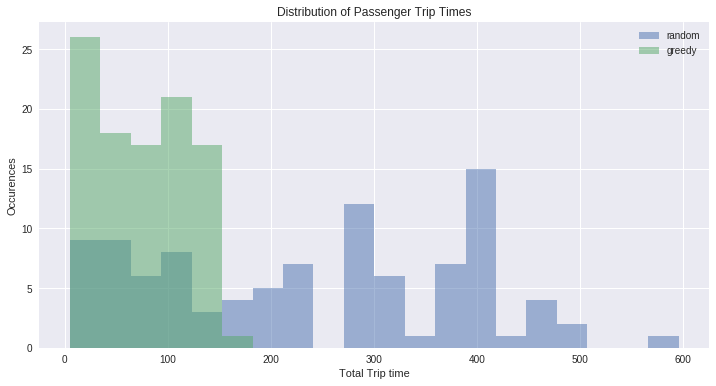
\includegraphics[width = 10cm]{Comparison.png}
\end{figure}

\newgeometry

Many assumptions were made which sacrificed realism in favor of model simplicity. We assumed, for example, that all passengers always made the correct decisions in pressing the buttons in the elevator, and always got off at the right floor. In our simulation, all passengers were initialized at once, instead of gradually initialized over time as would be expected of normal passenger behavior. These hypothetical passengers were also willing to stand in front of the elevator for an indefinitely long period of time and did not leave until they arrived at their destination. When they did arrive, passengers who got off the elevator and those who got onto the elevator did so using exactly 1 unit of time. 

\section*{Contributions to the Project}
Because of Oren's experience, he was essentially the de facto leader of our group. I seemed to have the second most experience, and would help others with the code, correcting some of Oren's mistakes when I spotted them, and gave suggestions for how I believe the code should be structured. An example of this was the decision to have the elevator work inside of the building class, and helping with coding and explaining the greedy strategy of the elevator. Specifically, the problem was how to choose the nearest floor which was a destination for passengers in the elevator.  The solution looked like this: 
 \begin{verbatim}
currentfloor = np.array(4)
destinations = np.array([3,5,9])

destinations[np.argmin(np.abs(currentfloor - destinations))]	
\end{verbatim}
 Which, in this case, would return 3, which is the nearest floor. 
 \section*{Things I learned}
 I learned about structuring classes and how to get various classes to communicate with each other. For example, one of the main problems we faced was how to transfer passengers from the floor of the building, which was in the Building class, to the elevator class itself, and we resolved this by passing the passengers as arguments into the elevator class, from which the elevator would have to extract their destinations by looking at which buttons inside the elevator were pressed.\\
 
 Another thing which I learned was the use of the \texttt{repr} method, which allowed the representation of the passenger to be of a more readable format. When debugging, it was extremely helpful to see what went wrong since each passenger was presented not as an object assigned to a space in memory, but something like ['from 0 to 1']. This was achieved through: 
 \begin{verbatim}
 def __repr__(self):
        return f'from {self.origin} to {self.destination}' 	
 \end{verbatim}

 
 









	
\end{document}
